\documentclass[book.tex]{subfiles}
\begin{document}
\label{chapter_software_architecture}
\section{About the Source Code}
Commander Keen series 1-3 and 4-6 source code is not available as the current owner Zenimax\footnote{June 24, 2009, it was announced that id Software had been acquired by ZeniMax Media (owner of Bethesda Softworks).} has, as of writing this book, no interest in selling intellectual properties. Luckily the ownership of Commander Keen: Keen Dreams was in the hands of Softdisk. In June 2013, developer Super Fighter Team licensed the game from Flat Rock Software, the then-owners of Softdisk, and released a version for Android devices. \\
The following September, an Indiegogo crowdfunding campaign was started to attempt to buy the rights from Flat Rock for US\$1500 in order to release the source code to the game and start publishing it on multiple platforms. The campaign did not reach the goal, but it's creator Javier Chavez made up the difference, and the source code was released under GNU GPL-2.0-or-later soon after.

\section{Getting the Source Code}
\par
The source code is made available via \cw{github.com}. It is important to take the the source code from shareware version 1.13, otherwise you run into issues due to incompatible map headers. To get the correct source code \\
\par
\tcode{keen13_github.txt}\\
\par
\section{First Contact}
Once downloaded via \cw{github} a folder 'keen' is created with all source files inside.
\cw{cloc.pl} is a tool which looks at every file in a folder and gathers statistics about source code. It helps for getting an idea of what to expect.\\
\par

\begin{minipage}{\textwidth}
\lstinputlisting[]{code/cloc.txt}
\end{minipage}

\par
 The code is 85\% in C with assembly\footnote{All the assembly in Keen is done with TASM (a.k.a Turbo Assembler by Borland). It uses Intel notation where the destination is before the source: \cw{instr} \cw{dest} \cw{source}.} for bottleneck optimizations and low-level I/O such as video or audio.\\
 \par
   Source lines of code (SLOC) is not a meaningful metric against a single codebase but excels when it comes to extracting proportions. Commander Keen with its 19,237 SLOC is very small compared to most software. \cw{curl} (a command-line tool to download url content) is 154,134 SLOC. Google's Chrome browser is 1,700,000 SLOC. Linux kernel is 15,000,000 SLOC.\\
 \par
\begin{figure}[H]
\centering
  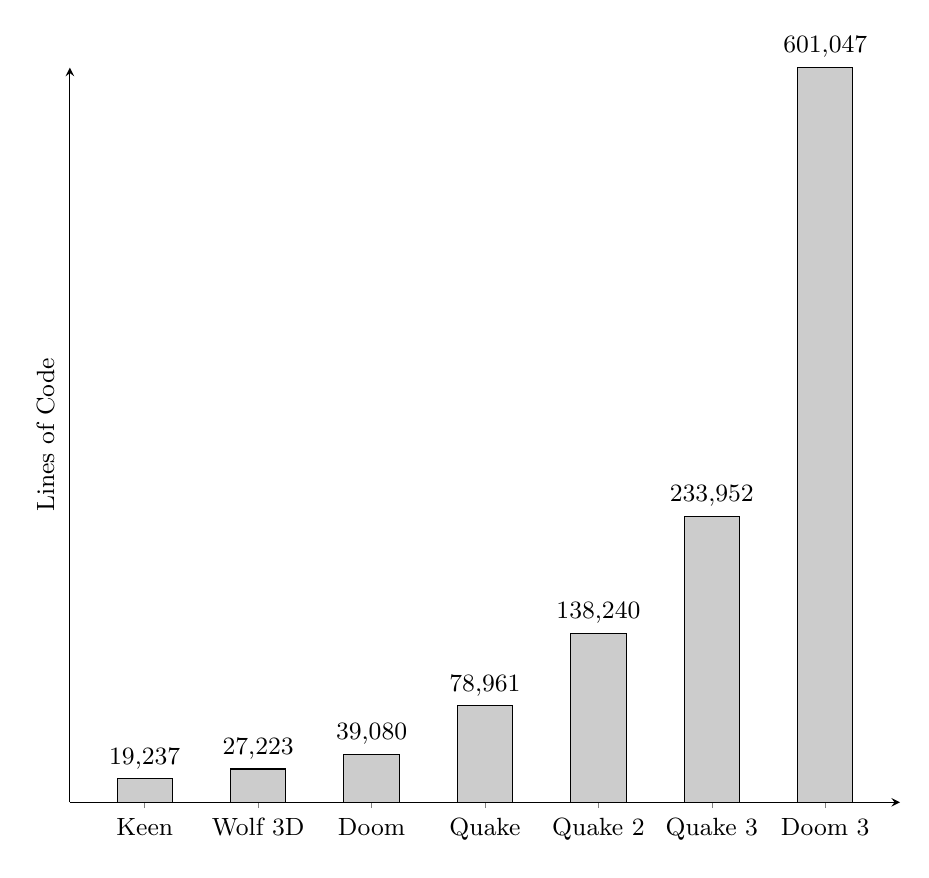
\begin{tikzpicture}[font=\small]
    \begin{axis}[
      width=\textwidth,
      height=0.9\textwidth,
      ybar=0.6\textwidth,
      bar width=20pt,
      ylabel={Lines of Code},
      ymin=0,
      ytick=\empty,
      xtick=data,
      axis x line=bottom,
      axis y line=left,
      enlarge x limits=0.11,
      symbolic x coords={Keen, Wolf 3D,Doom,Quake,Quake 2,Quake 3, Doom 3},
      xticklabel style={},
      yticklabel style={},
      nodes near coords={\pgfmathprintnumber[fixed,precision=0]\pgfplotspointmeta}
    ]
      \addplot[fill=black!20,draw=black] coordinates {
        (Keen, 19237)
        (Wolf 3D,27223)
        (Doom,39080)
        (Quake,78961)
        (Quake 2, 138240)
        (Quake 3, 233952)
        (Doom 3, 601047)
      };
    \end{axis}
   \end{tikzpicture} 
   \caption{Lines of code from id Software game engines.}
 \end{figure}
 
\par


 
The archive contains more than just source code; it also features:
\begin{itemize}
\item \codeword{static} folder: Static header files for loading assets (will be explained later).
\item \codeword{lscr} folder: Load and decompress Softdisk data files.
\item \codeword{README:} How to build the executable. 
\end{itemize}


\section{Compile source code}
Now let's start to compile the source code. To compile the code like it's 1990 you need the following software:
\begin{itemize}
\item Commander Keen source code.
\item DosBox.
\item The Compiler Borland C++ 3.1.
\item Commander Keen: Keen Dreams 1.13 shareware (for the assets).
\end{itemize}

After setting up the DosBox environment, with Borland C++ 3.1 installed (You can find a complete tutorial in "Let's compile like it's 1992" on \cw{fabiensanglard.net}) download the source code via github.\\

\par
Once you start DosBox and change directory to the \cw{keen} folder, first create the folder where we create our compiled object files.\\
\par
\tcode{mkdir.txt}\\
\par
Then we need to create the static \cw{OBJ} header files.\\
\par
\tcode{static.txt}\\
\par
Once the static object header files are created, move back to the \cw{keen} folder and open Borland C++. Open the \cw{kdreams.prj} project file. Before we can start compiling we need to set the correct directories. Select Options -> Directories and change the values as follow:
\begin{figure}[H]
\centering
  \fullimage{borland_directories.png}
\caption{Borland C++ 3.1 directory settings}
\end{figure}
\par
Now it's time to compile. Go to Compile -> Build all, and voila! The final step is to copy \cw{kdreams.exe} to the Keen shareware folder. Now you can play your compiled version of Commander Keen.
 \begin{figure}[H]
\centering
  \fullimage{borland_compile.png}
\caption{Commander Keen compiling}
\end{figure}
\par

\section{Big Picture}
The game engine is divided in three blocks:
\begin{itemize}
\item Control panel which lets users configure and start the game.
\item 2D game renderer where the users spend most of their time.
\item Sound system which runs concurrently with either the Menu or 2D renderer. 
\end{itemize}
The three systems communicate via shared memory. The renderer writes sound requests to the RAM (also making sure the assets are ready). These requests are read by the sound "loop". The sound system also writes to the RAM for the renderers since it is in charge of the heartbeat of the whole engine. The renderers update the screen according to the wall-time tracked by \cw{TimeCount} variable.
\par
\begin{figure}[H]
\centering
 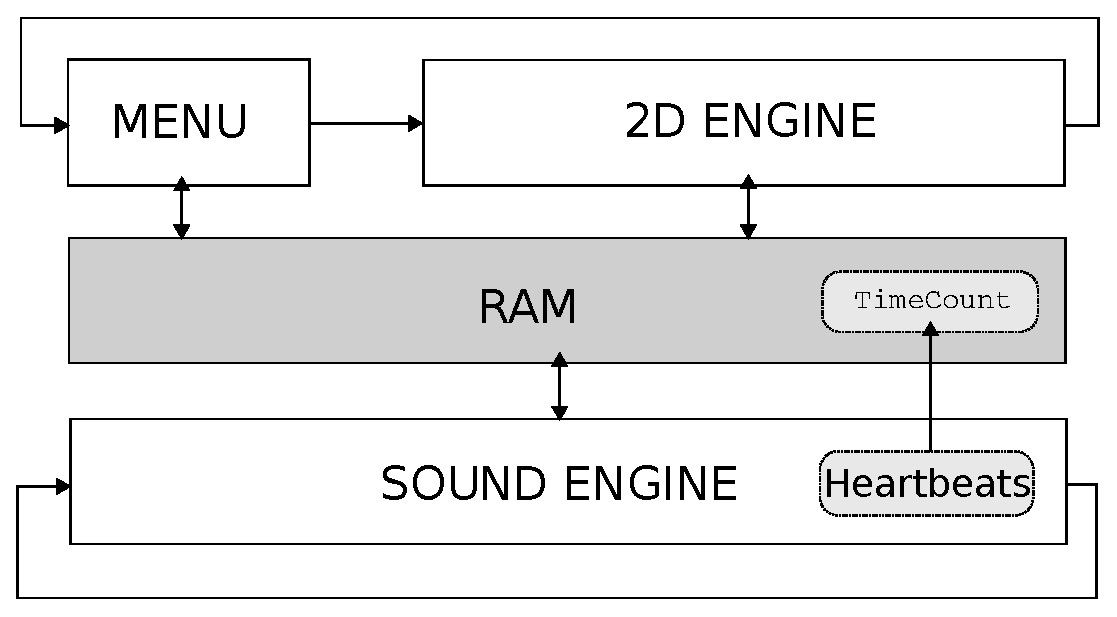
\includegraphics[width=\textwidth]{imgs/drawings/three_systems.eps}
 \caption{Game engine three main systems.}
 \end{figure}
 \par
 
\subsection{Unrolled Loop}
With the big picture in mind, we can dive into the code and unroll the main loop starting in \cw{void main()}. The control panel and 2D renderer are regular loops but due to limitations explained later, the sound system is interrupt-driven and therefore out of \cw{main}. Because of real mode, C types don't mean what people would expect from a 16-bit architecture.
\begin{itemize}
\item \cw{int} and \cw{word} are 16 bits.
\item \cw{long} and \cw{dword} are 32 bits.
\end{itemize}
\par
The first thing the program does is set the text color to light grey and background color to black.\\
\par
\begin{minipage}{\textwidth}
\lstinputlisting[language=C]{code/unrolled_loop_main.c}
\end{minipage}
\par

\par
In \cw{InitGame}, a valdation is performed to check if suficient memory is available and brings up all the managers.\\
\par
\begin{minipage}{\textwidth}
\lstinputlisting[language=C]{code/unrolled_loop_init.c}
\end{minipage}
\par
Then comes the core loop, where the menu and 2D renderer are called forever.

\begin{minipage}{\textwidth}
\lstinputlisting[language=C]{code/unrolled_loop_demoloop.c}
\end{minipage}
\par
\cw{PlayLoop} contains the 2D renderer. It is pretty standard with getting inputs, update screen, and render screen approach.\\
\par
\begin{minipage}{\textwidth}
\lstinputlisting[language=C]{code/unrolled_loop_playloop.c}
\end{minipage} \\
\par
 
The interrupt system is started via the Sound Manager in \cw{SDL\_SetIntsPerSec(rate)}. While there is a famous game development library called Simple DirectMedia Layer (SDL), the prefix \cw{SDL\_} has nothing to do with it. It stands for SounD Low level (Simple DirectMedia Layer did not even exist in 1991).\\
\par
The reason for interrupts is extensively explained in Chapter \ref{audio_and_heartbeat} "\nameref{audio_and_heartbeat}". In short, with an OS supporting neither processes nor threads, it was the only way to have something execute concurrently with the rest of the engine.\\
\par
An ISR (Interrupt Service Routine) is installed in the Interrupt Vector Table to respond to interrupts triggered by the engine. \\
\par
\begin{minipage}{\textwidth}
\lstinputlisting[language=C]{code/soundsystem_interrupt.c}
\end{minipage}
\par



\pagebreak
\section{Architecture}

The source code is structured in two layers. KD\_* files are high-level layers relying on low-level ID\_* sub-systems called Managers interacting with the hardware.\\
\par
\begin{figure}[H]
\centering
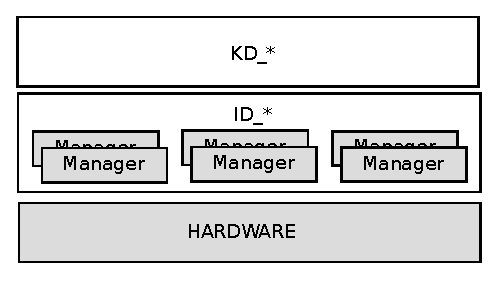
\includegraphics[width=\textwidth]{imgs/drawings/layers.eps} 
\caption{Commander Keen source code layers.}
 \end{figure}
 \par
There are six managers in total:\\

\begin{itemize}
	\item Memory
	\item Video
	\item Cache
	\item Sound
	\item User
	\item Input
\end{itemize}
\par
The KD\_ stuff was written specifically for Commander Keen while the ID\_ managers are generic and later re-used (with improvements) for newer ID games (Hovertank One, Catacomb 3-D and Wolf3D).

\begin{figure}[H]
\centering
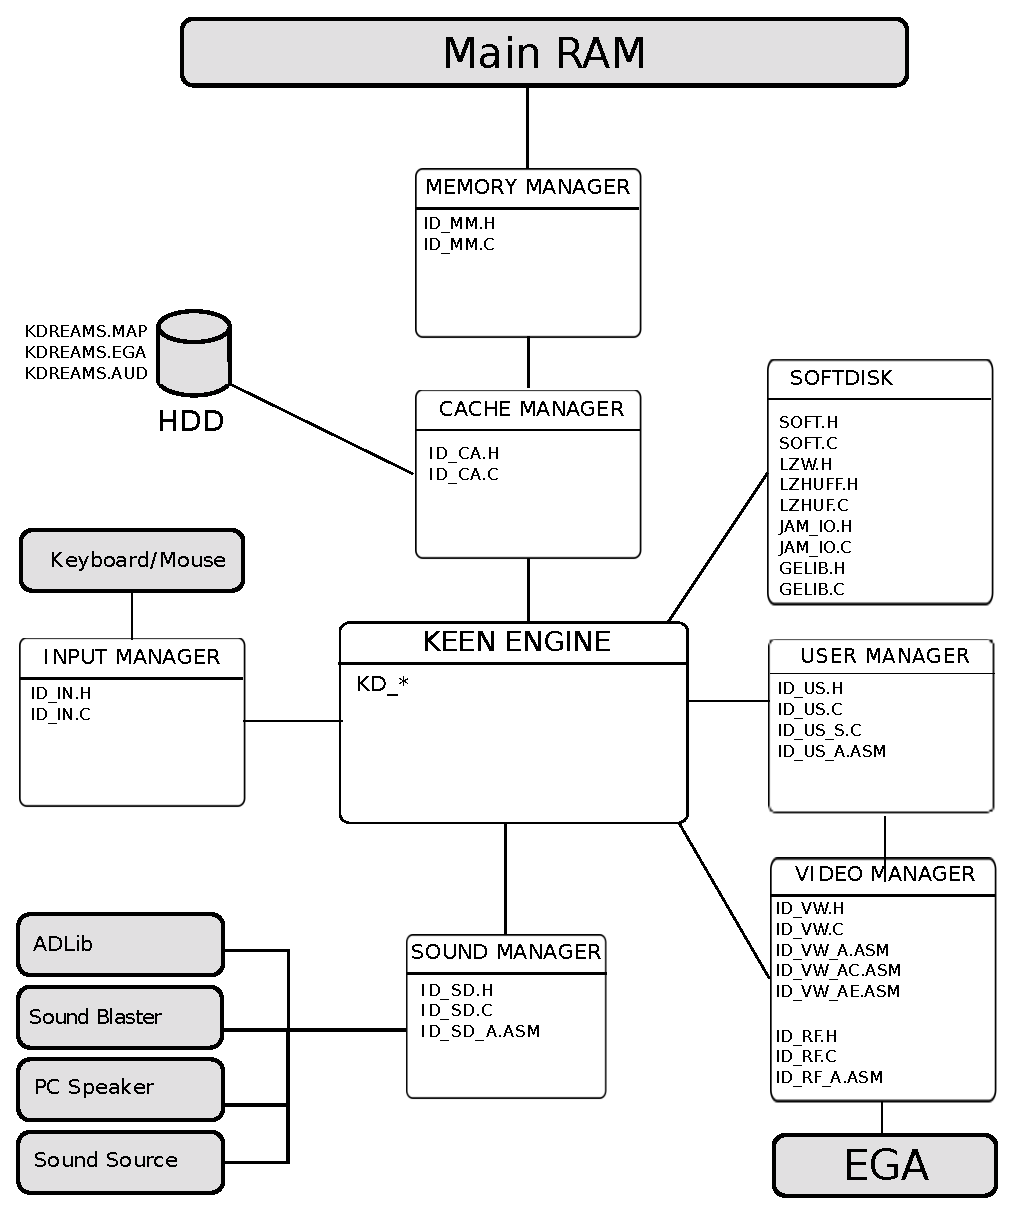
\includegraphics[width=\textwidth]{imgs/drawings/architecture.eps}
\caption{Architecture with engine and sub-systems (in white) connected to I/O (in gray).}
\label{fig:architecture}
\end{figure}
Next to the hard drives (HDD) you can see the assets packed as described in Chapter \ref{section:graphic_assets}.





\subsection{Memory Manager (MM)}
The engine does not rely on \cw{malloc} to manage conventional memory, as this can lead to fragmented memory and no way to compact free space. It has its own memory manager made of a linked list of "blocks" keeping track of the RAM. A block points to a starting point in RAM and has a size.\\
 \par
\lstinputlisting[language=C]{code/mm_block.c}
 \par
A block can be marked with attributes:
\begin{itemize}
\item \cw{LOCKBIT} : This block of RAM cannot be moved during compaction.
\item \cw{PURGEBITS} : Four levels available, 0= unpurgeable, 1= purgeable, 2= not used, 3= purge first.
\end{itemize}

The memory manager starts by allocating all available RAM via \cw{malloc}/\cw{farmalloc} and creates a \cw{LOCKED} block of size 1KiB at the end. The linked list uses two pointers: \cw{HEAD} and \cw{ROVER} which point to the second to last block.
 \par
\begin{figure}[H]
\centering
 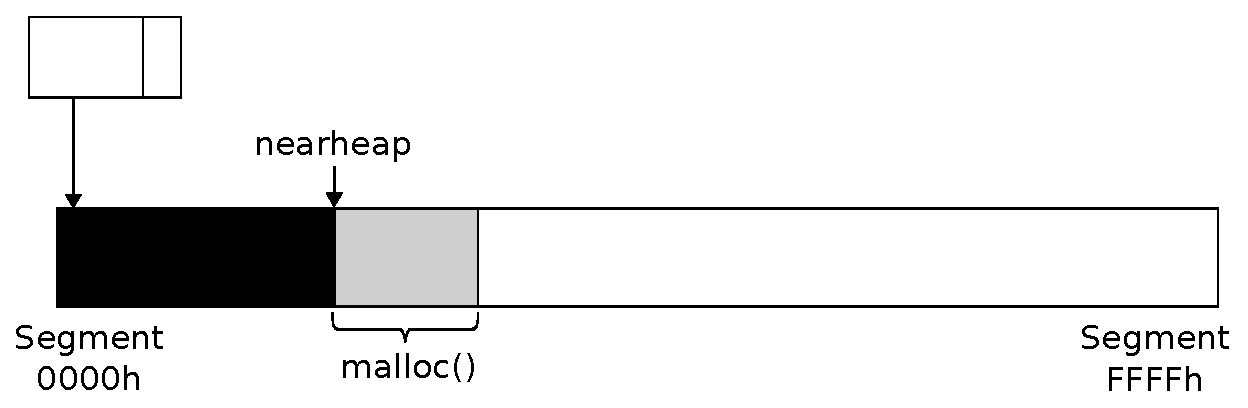
\includegraphics[width=\textwidth]{imgs/drawings/mm_start.eps}
 \caption{Initial memory manager state.}
 \end{figure}
 \par
 The engine interacts with the Memory Manager by requesting RAM (\cw{MM\_GetPtr}) and freeing RAM (\cw{MM\_FreePtr}). To allocate memory, the manager searches for "holes" between blocks. This can take up to three passes of increasing complexity:
\begin{enumerate}
\item After rover.
\item After head.
\item Compacting and then after rover.
\end{enumerate}
\par
  The easiest case is when there is enough space after the rover. A new node is simply added to the linked list and the rover moves forward. In the next drawing, three allocation requests have succeeded: \cw{A}, \cw{B} and \cw{C}.\\
  \par
\begin{figure}[H]
\centering
 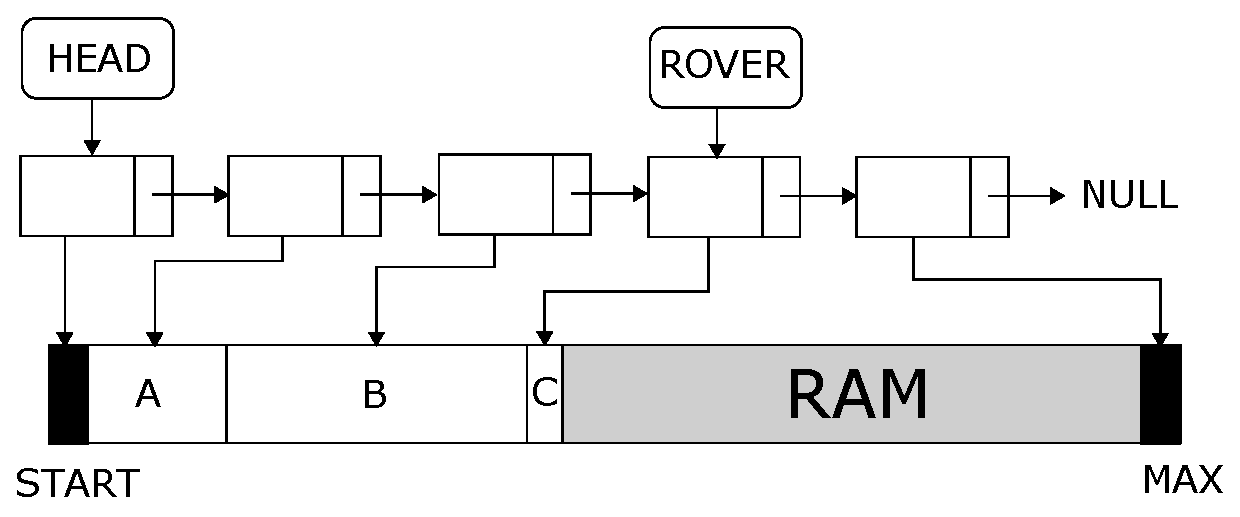
\includegraphics[width=\textwidth]{imgs/drawings/mm_after_rover.eps}
 \caption{MM internal state after three pass 1 allocations.}
 \end{figure}
 \par
Eventually the free RAM will be exhausted and the first pass will fail.
  \par
\begin{figure}[H]
\centering
 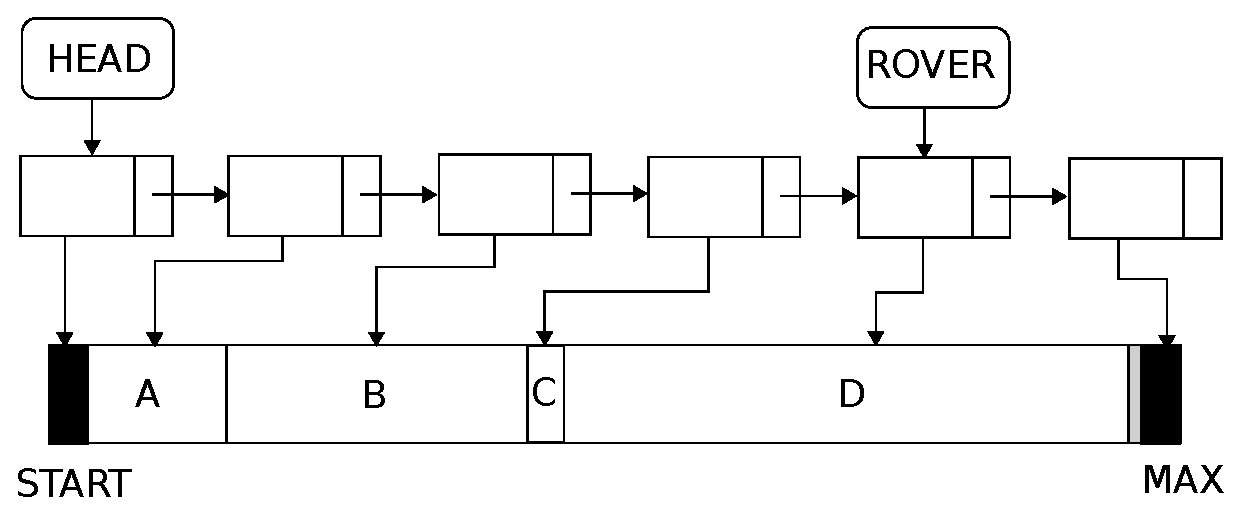
\includegraphics[width=\textwidth]{imgs/drawings/mm_before_rover.eps}
 \caption{Pass 1 failure: Not enough RAM after the ROVER.}
 \end{figure}
 \par
 If the first pass fails, the second pass looks for a "hole" between the head and the rover. This pass will also purge unused blocks. If for example block B was marked as \cw{PURGEABLE}, it will be deleted and replaced with the new block E. At this point fragmentation starts to appear (like if \cw{malloc} was used).\\
 \begin{figure}[H]
\centering
 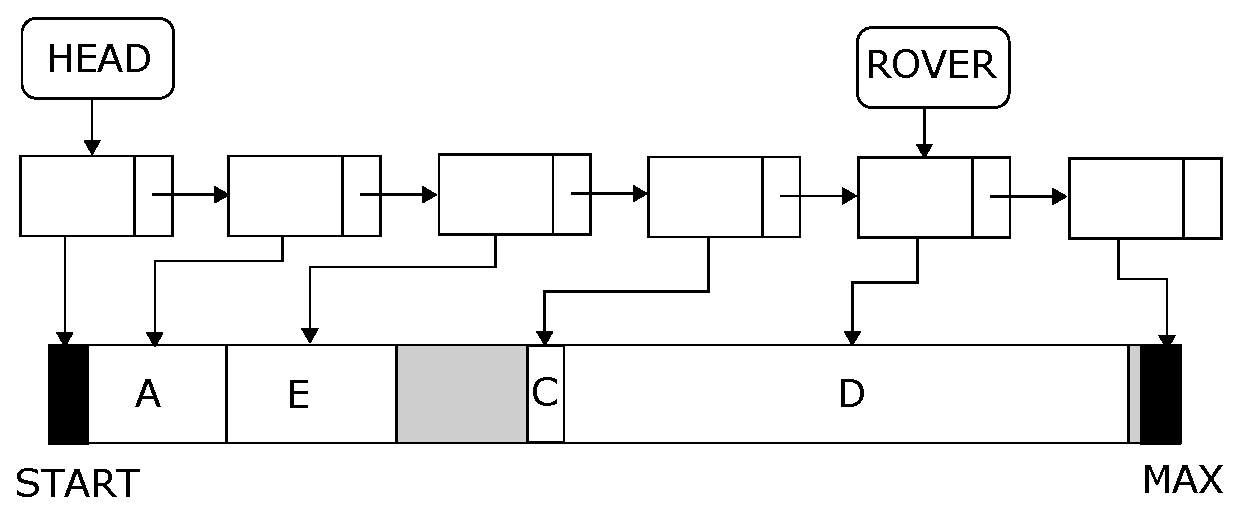
\includegraphics[width=\textwidth]{imgs/drawings/mm_after_head.eps}
 \caption{\cw{B} was purged. \cw{E} was allocated in pass 2.}
 \end{figure}
 \par
 If the first and second pass fail, there is no continuous block of memory large enough to satisfy the request. The manager will then iterate through the entire linked list and do two things: delete blocks marked as purgeable, and compact the RAM by moving blocks.
  \par
\begin{figure}[H]
\centering
 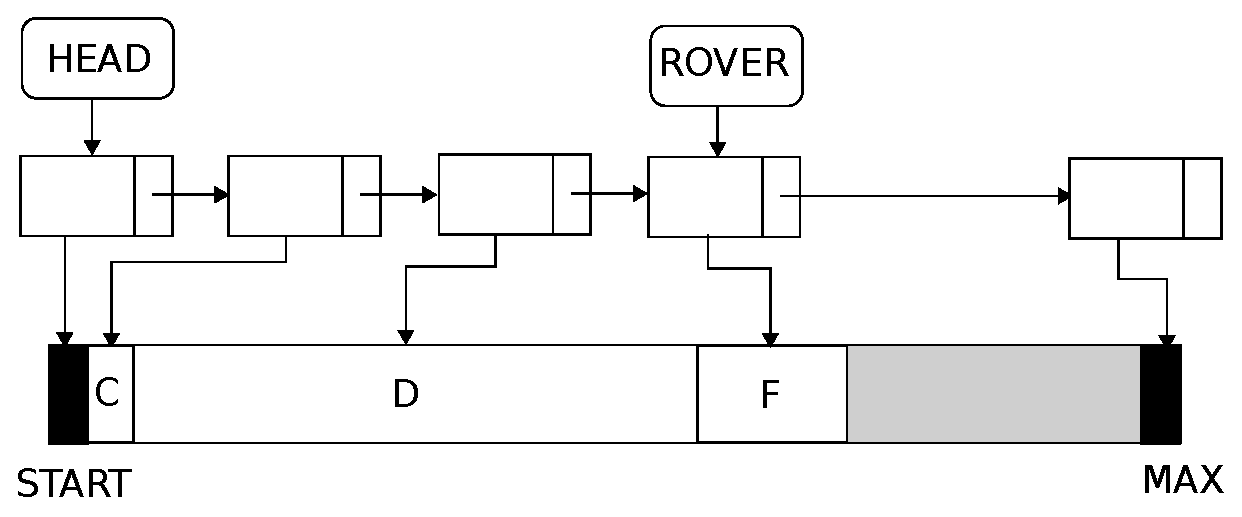
\includegraphics[width=\textwidth]{imgs/drawings/mm_compact.eps}
  \caption{\cw{A} and \cw{E} were purged. \cw{C} and \cw{D} compacted. \cw{F} allocated in pass3.}
 \end{figure}
 \par
But if memory is moved around, how do previous allocations still point to what they did before the compaction phase? Notice that a \cw{mmblockstruct} has a \cw{useptr} pointer which points to the owner of a block.  When memory is moved, the owner of the block is also updated.\\
\par
As some blocks are marked as \cw{LOCKED}, compacting can be disturbed. Upon encountering a locked block, compacting stops and the next block will be moved immediately after the locked block, even if there was space available between the last block and the locked block.\\
   \par
\begin{figure}[H]
\centering
 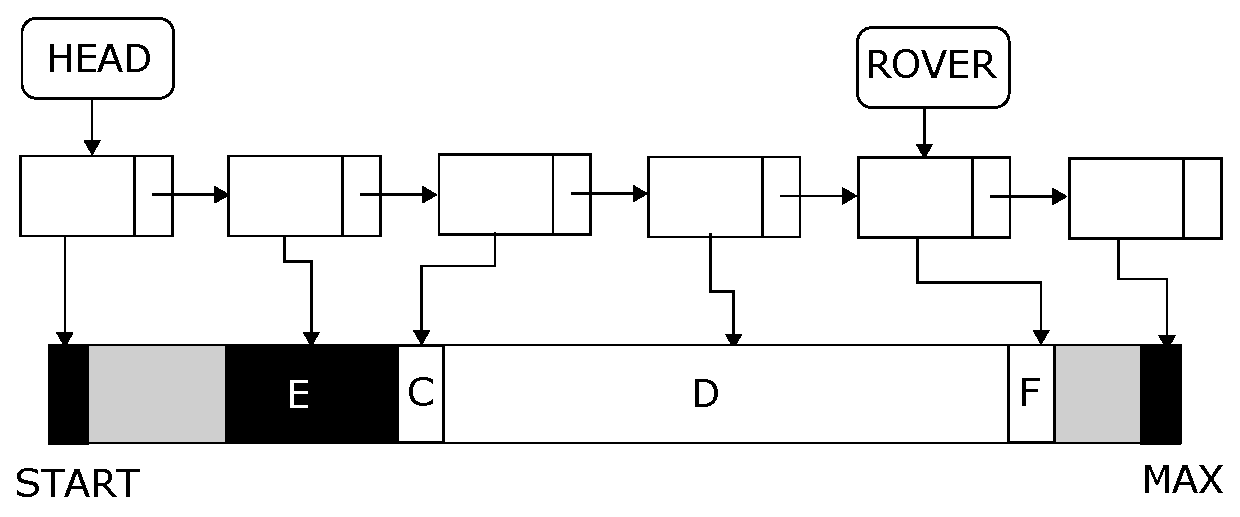
\includegraphics[width=\textwidth]{imgs/drawings/mm_bad_compact.eps}
 \caption{\cw{E} is locked and cannot be compacted.}
 \end{figure}
 \par
  In the above drawing, C was moved after E, even though it could have been moved before. Avoiding this waste would have made the memory manager more complicated, so the waste was deemed acceptable. Often in designing a component you have to be practical and establish a certain trade off between accuracy and complexity.\\
  \par
  
  
  


\subsection{Video Manager (VW \& RF)}
The video manager features two parts:
\begin{itemize}
\item The \cw{VW\_*} layer is made of both C and ASM, where the C functions abstract away EGA register manipulation via assembly routines. 
\item The \cw{RF\_*} layer is used to update tiles, and is also made both C and ASM code.
\end{itemize}
The video manager is described extensively in section \ref{section:adaptive_tile_refresh} on page \pageref{section:adaptive_tile_refresh}.
\par





\subsection{Cache Manager (CA)}
The cache manager is a small but critical component. It loads and decompresses maps, graphics and audio resources stored on the filesystem and makes them available in RAM. Assets of each kind are stored into three files: 
\begin{itemize}
	\item A header file containing the offset to allow translation from asset ID to byte offset in the data file.
	\item A compression dictionary to decompress each asset
	\item The data file containing the assets
\end{itemize}
 \par
 
Details of each asset file are explained in chapter \ref{section:programming}. The header and dictionary files are provided with the source code in the \cw{static} folder and contain \cw{*.KDR} extension. Both file types are hardcoded and required during compilation (they are converted into an \cw{OBJ} file using \cw{makeobj.c}). The data file containing the assets is not part of the source code and must be acquired via downloading the shareware version.
 All resources are compressed using a traditional huffman method for (de-)compression. \\
 \par
\begin{figure}[H]
\centering
 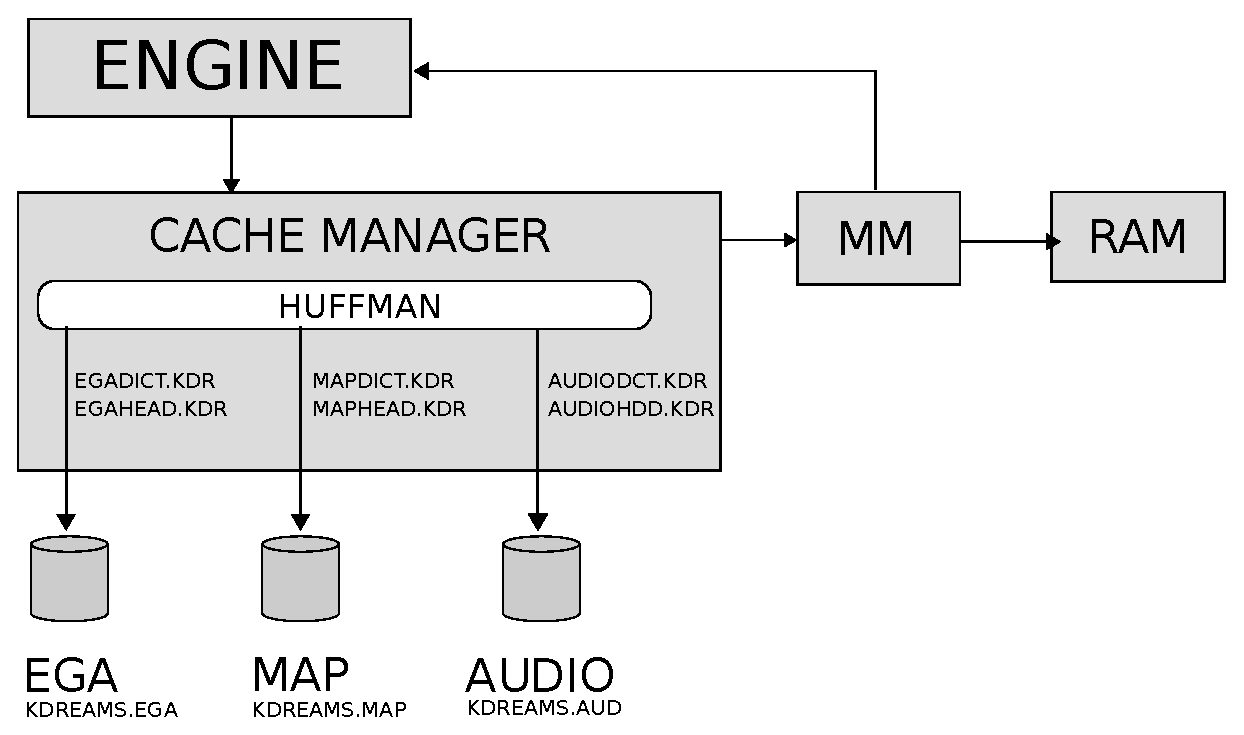
\includegraphics[width=\textwidth]{imgs/drawings/cache_manager_architecture.eps}
 \end{figure}
\pagebreak
To keep track of required assets, an array \cw{gr\_needed[]} is maintained to mark if an asset needs to be loaded from disk.
 \par
\lstinputlisting[language=C]{code/unrolled_mark_cache.c}
 \par
The function \cw{CA\_CacheMarks()} loads and decompress all required graphical assets from disk to memory. Since access and loading from disk is a slow process, the engine will try to load as much as possible assets in one go from the disk.
 \pagebreak
\lstinputlisting[language=C]{code/unrolled_load_cache.c}
 \par
 
 
 
\subsection{User Manager (US)} 
The user manager is responsible for text layout and control panels like loading and saving games, configure controls and setting sound device.\\
\par

Once we start the game, we move the display to EGA graphic mode \cw{0x0D}. Here we can't directly print characters on the screen anymore. So a key function of the User Manager is to print text for a given pixel location. When a high-level routine needs to draw a string, it is first passed to \cw{USL\_MeasureString} which does all measurement (e.g. height and total width of string) and then to \cw{USL\_DrawString} which passes this information to the Video Manager (\cw{VW\_DrawPropString}), which takes care of rendition.
In the graphic assets file the complete font is stored with the following information for each character:
\begin{itemize}
  \item The width of the character
  \item The location in memory where each character is stored as a bitmap
\end{itemize}
Each character has the same height of 10 pixels, where the width could vary as illustrated in Figure \ref{fig:text_bitmap}. 
\begin{figure}[H]
\centering
 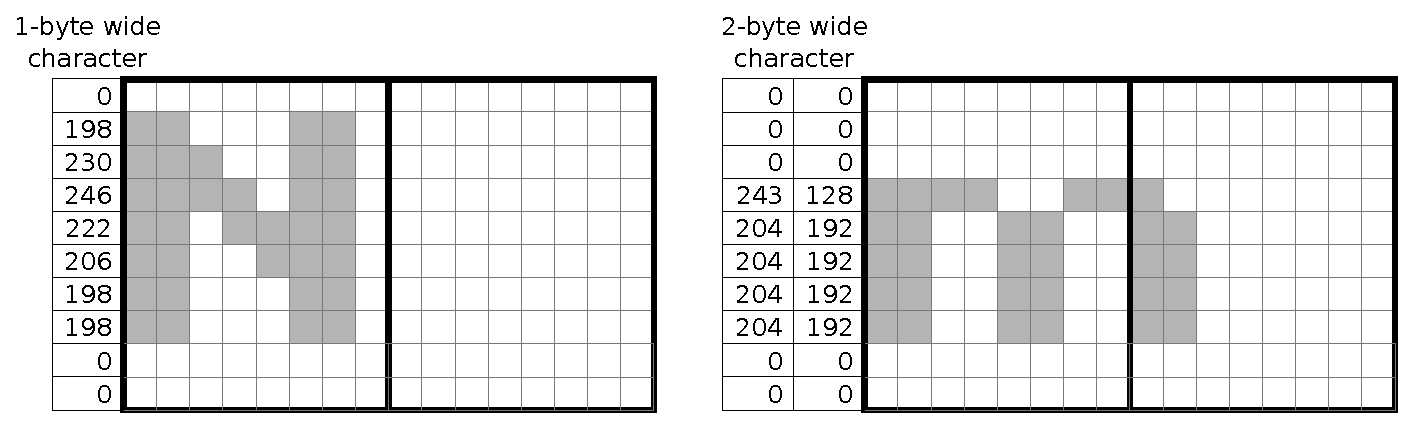
\includegraphics[width=\textwidth]{imgs/drawings/text_bitmap.eps}
 \caption{Character bitmaps of 'N' (7 bits wide) and 'm' (11 bits wide)}
 \label{fig:text_bitmap}
 \end{figure}
 \par
 
\subsection{Bitshifting}
\label{section:bitshifting}
As explained in section \ref{section:ega_memmap} on page \pageref{section:ega_memmap}, each 8 pixels are represented by 1 byte per memory bank. So how do we print a character which is not perfectly aligned with the memory layout? Here a trick of bit shift tabels is being used. \\
\par

The default table (\cw{shiftdata0}) is defined as integer (16 bits) and contains all values from 0-255. Now, we shift this entire table 1 bit to the right. We can translate the bit shift back into an integer and store these values again in a table (\cw{shiftdata1}). We can do this again when we shift another bit, until we cycled through the 8-bits. So at the end we have created 7 shift tables to fully cycle through 8-bits. In Figure \ref{fig:shiftttable} you see how the bitshift is working for the values '198'.
\begin{figure}[H]
\centering
 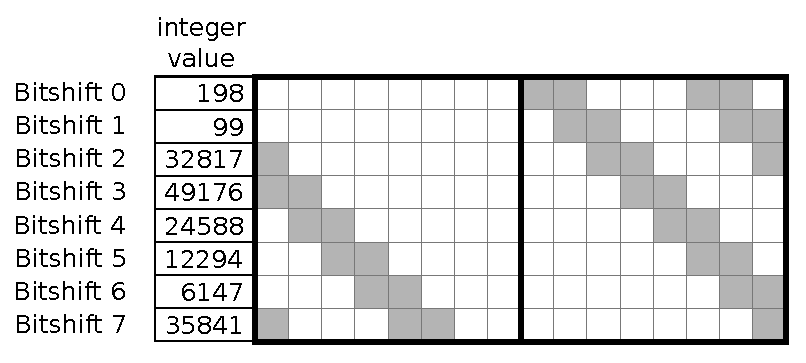
\includegraphics[width=0.8\textwidth]{imgs/drawings/shift_tables.eps}
 \caption{Right bitshift [0-7] for 198.}
 \label{fig:shiftttable}
 \end{figure}
 \par

Each bitshift table is generated in \cw{id\_vw\_a.asm} \\
\begin{minipage}{\textwidth}
  \lstinputlisting[basicstyle=\fontsize{7}{9}\selectfont]{code/unrolled_shift_table.c}
\end{minipage}
\label{wallclip_array}
\par
 

Now let's take the example of printing 'N', with an \cw{x} offset of 3 pixels. A simple lookup in \cw{shiftdata3} results in the 3-bit shifted 'N'. Note that you first display the low byte and then the high byte value. \\
\begin{figure}[H]
\centering
 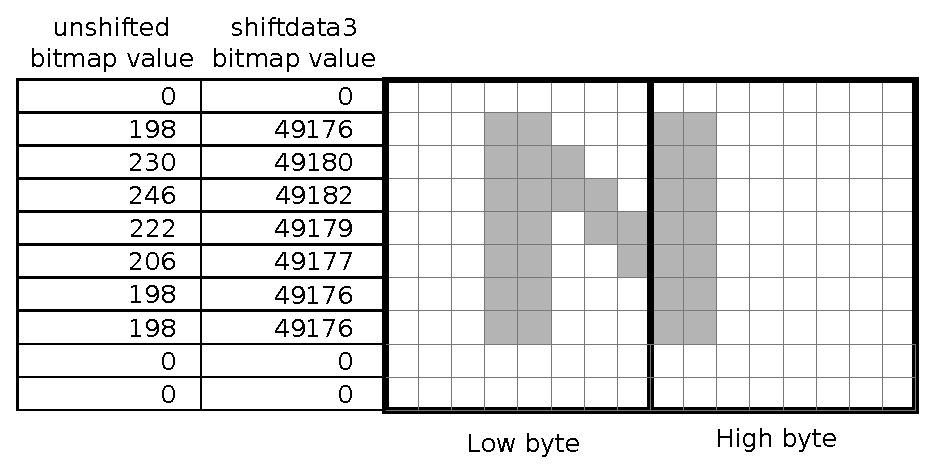
\includegraphics[width=\textwidth]{imgs/drawings/text_bitshift_N.eps}
 \caption{Bitshift 'N' over 3 bits using bit shift tables.}
 \label{fig:text_bitshift_N}
 \end{figure}
 \par

Once both bytes are copied to the data buffer, the buffer pointer is increased with the character width and then the next character is copied.  To avoid the next character overwrites the last high byte in the buffer, every low byte is added to the last high byte by applying a logical \cw{OR}-operation.

\begin{minipage}{\textwidth}
  \lstinputlisting[language={[x86masm]Assembler}]{code/unrolled_ShiftPropChar.asm}
\end{minipage}
\par
\subsection{Sound Manager (SD)}
The Sound Manager abstracts interaction with all four sound systems supported: PC Speaker, AdLib, Sound Blaster, and Disney Sound Source. It is a beast of its own since it doesn't run inside the engine. Instead it is called via IRQ at a much higher frequency than the engine (the engine runs at a maximum 70Hz, while the sound manager ranges from 140Hz to 700Hz). It must run quickly and is therefore written in small and fast routines.\\
 \par
\begin{figure}[H]
\centering
 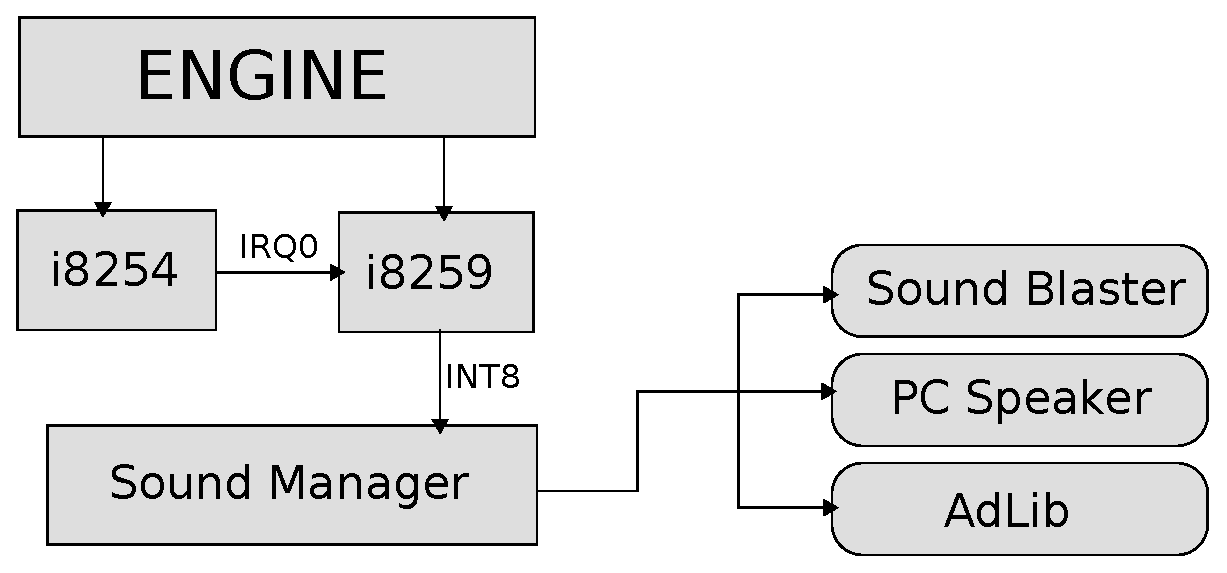
\includegraphics[width=\textwidth]{imgs/drawings/sound_manager_architecture.eps}
 \caption{Sound system architecture.}
 \end{figure}
 \par
The sound manager is described extensively in the "Sound and Music" section.





\subsection{Input Manager (IN)}
The input manager abstracts interactions with joystick, keyboard, and mouse. It features the boring boilerplate code to deal with PS/2, Serial, and DA-15 ports, with each using their own I/O addresses.

\subsection{Softdisk files}
The only function for the softdisk files is to load and show the intro screen bitmap, using \cw{LoadLIBShape} from soft.c. However, most of the functions in these files are actually not used and therefor not further discussed in this book.
\pagebreak



\section{Startup}
As the game engine starts, it will first load the memory manager. Then it will check if there is at least 335KiB of RAM available. If not, it gives  a warning, but you can continue with the game. But most likely somewhere soon the game will either crash or receives and "Out of memory" error.\\
\par
After succesfully starting the game the intro image is diplayed, which is a Deluxe PaintBitmap image (*.LBM). After the user has hit any key, the intro image is unloaded from RAM to make more room for runtime and the control panel is shown.\\
\begin{figure}[H]
\centering
\fullimage{Keen_intro_screen.png}
\caption{Keen Dreams intro screen}
\end{figure}
\pagebreak
\end{document}
